
\documentclass[a4paper]{article}
\usepackage[hmargin=2cm,vmargin=2cm]{geometry}


\pagestyle{plain}

\usepackage{amssymb,amsthm,amsfonts,longtable, comment,array, ifpdf, hyperref,cite,url}
\usepackage{graphicx}
\newtheorem{theorem}{Theorem}
\newtheorem{lemma}{Lemma}
\newcommand{\Tag}{\mathrm{Tag}}


% *** MATH PACKAGES ***
%
\usepackage[cmex10]{amsmath}




% *** SPECIALIZED LIST PACKAGES ***
%
\usepackage{algorithmic}





\begin{document}

%FINISHED

\title{\textsf{Argon2: the memory-hard function for password hashing and other applications}}

\author{Designers: Alex Biryukov, Daniel Dinu,  and Dmitry Khovratovich\\University of Luxembourg, Luxembourg
\\[10pt]
%Submitters: Alex Biryukov and Dmitry Khovratovich
%\\
{\tt alex.biryukov@uni.lu, dumitru-daniel.dinu@uni.lu, khovratovich@gmail.com}\\[10 pt]
\url{https://www.cryptolux.org/index.php/Argon2}\\
\url{https://github.com/P-H-C/phc-winner-argon2}\\
\url{https://github.com/khovratovich/Argon2}\\[10pt]
Version 1.3 of Argon2: PHC release}

\maketitle

\tableofcontents

\section{Introduction}

Passwords, despite all their drawbacks, remain the primary form of authentication on various web-services. Passwords are usually stored in a hashed form in a server's database. These databases are quite often captured by the adversaries,  who then apply dictionary attacks since passwords tend to have low entropy. Protocol designers use a number of tricks to mitigate these issues. Starting from the late 70's, a password is hashed together with a random \emph{salt} value to prevent detection of identical passwords across different users and services. The hash function computations, which became faster and faster due to Moore's law have been called multiple times to increase the cost of password trial for the attacker.

 In the meanwhile, the password crackers migrated to new architectures, such as FPGAs, multiple-core GPUs and dedicated ASIC modules, where the amortized cost of a multiple-iterated hash function is much lower. It was quickly noted that these new environments are great when the computation is almost memoryless, but they experience difficulties when  operating on a large amount of memory. The defenders responded by designing \emph{memory-hard} functions, which require a large amount of memory to be computed, and impose computational penalties if less memory is used. The password hashing scheme \textsf{scrypt}~\cite{percival2009stronger} is an instance of such function.

Memory-hard schemes also have other applications. They can be used for key derivation from low-entropy sources. Memory-hard schemes are also welcome in cryptocurrency designs~\cite{litecoin} if a creator wants to demotivate the use of GPUs and ASICs for mining and promote the use of standard desktops.

\paragraph{Problems of existing schemes} A trivial solution for password hashing is a keyed hash function such as HMAC. If the protocol designer prefers hashing without secret keys to avoid all the problems with key generation, storage, and update, then he has few alternatives: the generic mode PBKDF2, the Blowfish-based \textsf{bcrypt}, and \textsf{scrypt}. Among those, only 
\textsf{scrypt} aims for high memory, but the existence of a trivial time-memory tradeoff~\cite{ForlerLW14} allows compact implementations with the same energy cost.

Design of a memory-hard function proved to be a tough problem. Since early 80's it has been known that many cryptographic problems that seemingly require large memory actually allow for a time-memory tradeoff~\cite{hellman1980cryptanalytic}, where the adversary can trade memory for time and do his job on fast hardware with low memory. In application
to password-hashing schemes, this means that the password crackers can still be implemented on a dedicated hardware even though at some additional cost. 

Another problem with the existing schemes is their complexity. The same \textsf{scrypt} calls a stack of subprocedures, whose design rationale has not been fully motivated (e.g, \textsf{scrypt} calls SMix, which calls ROMix, which calls BlockMix, which calls Salsa20/8 etc.).  It is hard to analyze and, moreover, hard to achieve confidence. Finally, it is not flexible in separating time and memory costs. 
At the same time, the story of cryptographic competitions~\cite{robshaw2008new,sha3} has demonstrated that
the most secure designs come with simplicity, where every element is well motivated and a cryptanalyst has as few entry points as possible.

The  Password Hashing Competition, which started in 2014,  highlighted the following problems:
\begin{itemize}
  \item Should the memory addressing (indexing functions) be input-independent or input-dependent, or hybrid? The first type of schemes, where the memory read location are known in advance, is immediately vulnerable to time-space tradeoff attacks,
 since an adversary can precompute the missing block by the time it is needed~\cite{trade-att}. In turn, the input-dependent schemes are vulnerable to side-channel attacks~\cite{RistenpartTSS09}, as the timing information allows for much faster password search.
  \item Is it better to fill more memory but suffer from time-space tradeoffs, or make more passes over the memory to be more robust? This question was quite difficult to answer due to absence of generic tradeoff tools, which would analyze the security against tradeoff attacks, and the absence of unified metric to measure adversary's costs.
          \item How should the input-independent addresses be computed? Several seemingly secure options have been attacked~\cite{trade-att}.
  \item How large a single memory block should be? Reading smaller random-placed blocks is slower (in cycles per byte) due to the spacial locality principle of the CPU cache. In turn, larger
  blocks are difficult to process due to the limited number of long registers.
  \item If the block is large, how to choose the internal compression function? Should it be cryptographically secure or more lightweight, providing only basic mixing of the inputs? Many candidates simply proposed an iterative construction  and argued against cryptographically strong transformations.

      \item How to exploit multiple cores of modern CPUs, when they are available? Parallelizing calls to the hashing function without any interaction is subject  to simple tradeoff attacks.
\end{itemize}

\paragraph{Our solution} We offer a hashing scheme called  \textsf{Argon2}.
 \textsf{Argon2} summarizes the state of the art in the design of memory-hard functions. It is a streamlined and simple design. It aims at the highest memory filling rate and effective use of multiple computing units, while still
providing defense against tradeoff attacks. \textsf{Argon2} is optimized for the x86 architecture and exploits the cache and memory organization of the recent Intel and AMD processors. \textsf{Argon2} has two variants: \textsf{Argon2d} and \textsf{Argon2i}. \textsf{Argon2d} is faster and uses data-depending memory access, which makes it suitable for cryptocurrencies and applications with no threats from side-channel timing attacks. \textsf{Argon2i} uses data-independent memory access, which is preferred for password hashing and password-based key derivation. \textsf{Argon2i} is slower as it makes more passes over the memory to protect from tradeoff attacks.


We recommend \textsf{Argon2} for the applications that aim for high performance. Both versions of \textsf{Argon2} allow to fill 1 GB of RAM in a fraction of second, and smaller amounts even faster. It scales easily to the arbitrary number of parallel computing units. Its design is also optimized for clarity to ease analysis and implementation.

Our scheme provides more features and better tradeoff resilience than pre-PHC designs and equals in performance with the  PHC finalists~\cite{broz15}. 

\section{Definitions}

\subsection{Motivation}\label{sec:costs}
We aim to maximize the cost of password cracking on ASICs. There can be different approaches to measure this cost, but we turn to one of the most popular -- the time-area product~\cite{Thompson79,BernsteinL13}. We assume that the password $P$ is hashed with salt $S$ but without secret keys, and the hashes may leak to the adversaries together with salts:
$$
\begin{aligned}
\mathrm{Tag} &\leftarrow \mathcal{H}(P,S);\\
\mathrm{Cracker} &\leftarrow \{(\mathrm{Tag}_i, S_i)\}.
\end{aligned}
$$

In the case of the password hashing, we suppose that the defender allocates certain amount of time (e.g., 1 second) per password and a certain number of CPU cores (e.g., 4 cores). Then he hashes the password using the maximum amount $M$ of memory. This memory size translates to certain ASIC area $A$. The running ASIC time $T$ is determined by the length of the longest computational chain and by the ASIC memory latency.
Therefore, we maximize the value $AT$. The other usecases follow a similar procedure. 

Suppose that an ASIC designer that wants to reduce the memory and thus the area wants to compute $\mathcal{H}$ using $\alpha M$ memory only for some $\alpha<1$. Using some tradeoff specific to $\mathcal{H}$, he has to spend $C(\alpha)$ times as much computation and his running time increases by at least the factor $D(\alpha)$. Therefore, the maximum possible gain $\mathcal{E}$ in the time-area product is 
$$
\mathcal{E}_{max}= \max_{\alpha}\frac{1}{\alpha D(\alpha)}.
$$
The hash function is called \emph{memory-hard} if $D(\alpha) >1/\alpha$ as $\alpha\rightarrow 0$. Clearly, in this case the time-area product does not decrease. Moreover, the following aspects may further increase it:
\begin{itemize}
\item Computing cores needed to implement the $C(\alpha)$ penalty may occupy significant area.
\item If the tradeoff requires significant communication between the computing cores, the memory bandwidth limits may impose additional restrictions on the running time.
\end{itemize}

In the following text, we will not attempt to  estimate  time and area with large precision. However, an interested reader may use the following implementations as reference:
 \begin{itemize}
   \item The 50-nm DRAM implementation~\cite{giridhar2013dram} takes 550 mm${}^2$ per GByte;
   \item The Blake2b implementation in the 65-nm process should take about 0.1 mm${}^2$ (using Blake-512 implementation in~\cite{gurkaynak2012sha3});
   \item The maximum memory bandwidth achieved by modern GPUs is around 400 GB/sec.
 \end{itemize}
 
 \subsection{Model for memory-hard functions}
 
 The memory-hard functions that we explore use the following mode of operation. The memory array $B[]$ is filled with the   compression function $G$:

 \begin{equation}\label{eq:class}
\begin{array}{rl}
B[0] &= H(P,S);\\
\text{for $j$ }&\text{from 1  to } t\\
  &B[j] = G \bigl(B[\phi_1(j)] ,  B[\phi_2(j)] ,\cdots , B[\phi_k(j)]\bigr),
\end{array}
\end{equation}
where $\phi_i()$ are some \emph{indexing functions}.


We distinguish two types of indexing functions:
\begin{itemize}
  \item Independent of the password and salt, but possibly dependent on other public parameters (thus called \emph{data-independent}). The addresses can be calculated by the memory-saving adversaries. We suppose that the dedicated hardware can handle parallel memory access, so that the  cracker can prefetch the data from the memory. Moreover, if she implements a time-space tradeoff, then the missing blocks can be also precomputed without losing time. Let the single $G$ core occupy the area equivalent to the $\beta$ of the entire memory. Then if we use $\alpha M$ memory, then the  gain in the time-area product is
  $$
  \mathcal{E}(\alpha) = \frac{1}{\alpha + C(\alpha)\beta}.
  $$
  \item Dependent on the password (\emph{data-dependent}), in our case: $\phi(j) = g(B[j-1])$. This choice prevents the adversary from prefetching and precomputing missing data. The adversary figures out what he has to recompute only at the time the element is needed. If an element is recomputed as a tree of $F$ calls of average depth $D$, then the total processing time is multiplied by $D$. The   gain in the time-area product is
  $$
  \mathcal{E}(\alpha) = \frac{1}{(\alpha + C(\alpha)\beta)D(\alpha)}.
  $$
\end{itemize}


 The maximum bandwidth $Bw_{max}$ is a hypothetical upper bound on the memory bandwidth on the adversary's architecture. Suppose that for each call to $G$ an adversary has to load
  $R(\alpha)$ blocks from the memory on average. Therefore,  the adversary can keep the execution time the same as long as
 $$
 R(\alpha) Bw \leq Bw_{max},
 $$
 where $Bw$ is the bandwidth achieved by a full-space implementation. In the tradeoff attacks that we apply the following holds:
   $$
   R(\alpha)  = C(\alpha).
   $$



\section{Specification of Argon2}

There are two flavors of \textsf{Argon2}\ -- \textsf{Argon2d} and \textsf{Argon2i}. The former one uses data-dependent memory access to thwart tradeoff attacks. However, this makes it vulnerable for side-channel attacks, so \textsf{Argon2d} is recommended primarily for cryptocurrencies and backend servers. \textsf{Argon2i} uses data-independent memory access, which is recommended for password hashing and password-based key derivation.

\subsection{Inputs}

\textsf{Argon2}\ has two types of inputs: primary inputs and secondary inputs, or parameters. Primary inputs are message $P$ and nonce $S$, which are password and salt, respectively, for the password hashing. Primary inputs must always be given by the user such that
\begin{itemize}
  \item Message $P$ may have any length from $0$ to $2^{32}-1$ bytes;
  \item Nonce $S$ may have any length from $8$ to $2^{32}-1$ bytes (16 bytes is recommended for password hashing).
\end{itemize}
 Secondary inputs have the following restrictions:
\begin{itemize}
  \item Degree of parallelism $p$ determines how many independent (but synchronizing) computational chains can be run.  It may take any integer value from 1 to $2^{24}-1$.
  \item Tag length $\tau$ may be any integer number of bytes from 4 to $2^{32}-1$.
  \item Memory size $m$ can be any integer number of kilobytes from $8p$ to $2^{32}-1$. The actual number of blocks is $m'$, which is $m$ rounded down to the nearest multiple of $4p$. 
  \item Number of iterations $t$ (used to tune the running time independently of the memory size) can be any integer number from 1 to $2^{32}-1$;
  \item Version number $v$ is one byte $0x13$;
  \item Secret value $K$ (serves as key if necessary, but we do not assume any key use by default) may have any length from $0$ to $2^{32}-1$ bytes.
  \item Associated data $X$ may have any length from $0$ to $2^{32}-1$ bytes.
  \item Type $y$ of \textsf{Argon2}: 0 for  \textsf{Argon2d}, 1 for \textsf{Argon2i}, 2 for \textsf{Argon2id}.
\end{itemize}

\textsf{Argon2}\ uses internal compression function ${G}$ with two 1024-byte inputs and a 1024-byte output, and internal hash function ${H}$. Here ${H}$ is the Blake2b hash function, and ${G}$ is based on  its internal permutation. The mode of operation of \textsf{Argon2} is quite simple when no parallelism is used: function ${G}$ is iterated $m$ times. At step $i$ a block with index $\phi(i)<i$ is taken from the memory (Figure~\ref{fig:generic}), where $\phi(i)$ is either determined by the previous block in \textsf{Argon2d}, or is a fixed value in \textsf{Argon2i}.



\begin{figure}[ht]
  \ifpdf
\begin{center}
  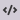
\includegraphics[scale=0.6]{pics/generic.pdf}
  \caption{Argon2 mode of operation with no parallelism. }\label{fig:generic}
\end{center}
\fi
  \end{figure}

\subsection{Operation}

\textsf{Argon2}\ follows the extract-then-expand concept. First, it extracts entropy from message and nonce by hashing it.  All the other parameters are also added to the input. The variable length inputs $P,S,K,X$  are prepended with their lengths:
$$
%H_0 = \mathcal{H}(p,\tau,m,t,v,y,\langle P \rangle,P,\langle S \rangle,S,\langle K \rangle,K, \langle X \rangle,X).
H_0 = H(p,\tau,m,t,v,y,\langle P \rangle,P,\langle S \rangle,S,\langle K \rangle,K, \langle X \rangle,X).
$$
Here $H_0$ is 64-byte value, and the parameters $p,\tau,m,t,v,y,
\langle P \rangle,\langle S \rangle, \langle K \rangle,\langle X \rangle$ are treated as little-endian 32-bit integers.

\textsf{Argon2}\ then fills the memory with $m' = \lfloor \frac{m}{4p} \rfloor\cdot 4p$ 1024-byte blocks. For tunable parallelism with $p$ threads, the memory is organized in a matrix $B[i][j]$ of blocks
with $p$ rows (\emph{lanes}) and $q=m'/p$ columns. We denote the block produced in pass $t$ by $B^t[i][j],t>0$. Blocks are computed as follows:
\begin{align*}
B^1[i][0] &= H'(H_0||\underbrace{0}_{\text{4 bytes}}||\underbrace{i}_{\text{4 bytes}}),\quad 0 \leq i < p; \\
B^1[i][1] &= H'(H_0||\underbrace{1}_{\text{4 bytes}}||\underbrace{i}_{\text{4 bytes}}),\quad 0 \leq i < p;\\
B^1[i][j] &= G(B^1[i][j-1], B^1[i'][j']),\quad 0 \leq i < p,\; 2\leq j <q.
\end{align*}
where block index $[i'][j']$ is determined differently for \textsf{Argon2d/2ds} and \textsf{Argon2i},  $G$ is the compression function, and $H'$ is a variable-length hash function built upon $H$. Both $G$ and $H'$ will be fully defined in the further text. 

If $t>1$, we repeat the procedure, but we XOR the new blocks to the old ones instead of overwriting them. 
%The first two blocks of a lane are now computed in the same way:
\begin{align*}
B^t[i][0] &=G(B^{t-1}[i][q-1], B[i'][j']) \oplus B^{t-1}[i][0];\\
B^t[i][j] &= G(B^{t}[i][j-1], B[i'][j'])\oplus B^{t-1}[i][j].
\end{align*}
Here the block $B[i'][j']$ may be either $B^t[i'][j']$ for $j'<j$ or $B^{t-1}[i'][j']$ for $j>j'$.

After we have done  $T$ iterations over the memory, we compute the final block $B_{\mathrm{final}}$ as the XOR of the last column:
$$
B_{\mathrm{final}} = B^T[0][q-1] \oplus B^T[1][q-1]\oplus \cdots\oplus B^T[p-1][q-1].
$$
Then we apply $H'$ to $B_{\mathrm{final}}$ to get the output tag.
$$
\text{Tag} \leftarrow H'(B_{\mathrm{final}}).
$$


\paragraph{Variable-length hash function.} Let $H_x$ be a hash function with $x$-byte output (in our case $H_x$ is Blake2b, which supports $1\leq x \leq 64$). We define $H'$ as follows. Let $V_i$ be a 64-byte block, and  $A_i$ be its first 32 bytes,
and $\tau<2^{32}$ be the 32-bit tag length (viewed little-endian) in bytes. 
Then we define
$$
\begin{array}{rl}
\text{if }\tau \leq 64&\\& H'(X) \overset{\text{def}}{=} H_{\tau}(\tau ||X).\\
\text{else}&\\
& r = \lceil\tau/32\rceil-2;\\
&V_1\leftarrow H_{64}(\tau||X);\\
&V_2 \leftarrow H_{64}(V_1);\\
&\cdots\\
&V_r  \leftarrow H_{64}(V_{r-1}),\\
&V_{r+1} \leftarrow H_{\tau - 32r}(V_{r}).\\
&H'(X) \overset{\text{def}}{=} A_1||A_2||\ldots A_r||V_{r+1}.
\end{array}
$$

 \begin{figure}[ht]
  \ifpdf
\begin{center}
  \includegraphics[scale=0.5]{pics/argon2-par.pdf}
  \caption{Single-pass \textsf{Argon2} with $p$ lanes and 4 slices. }\label{fig:argon2}
\end{center}
\fi
  \end{figure}

\subsection{Indexing}\label{sec:index}

To enable parallel block computation, we further partition the memory matrix into  $S=4$ vertical \emph{slices}. The intersection of a slice and a lane is a \emph{segment} of length $q/S$.  Segments of the same slice
  are computed in parallel, and may not reference blocks from each other. All other blocks can be referenced, and now we explain the procedure in detail.

\paragraph{Getting two 32-bit values.} In Argon2d we select  the first 32 bits of  block $B[i][j-1]$ and denote this value by $J_1$. Then we take the next 32 bits of $B[i][j-1]$ and denote this value by $J_2$. In \textsf{Argon2i} we run $G^2$ --- the 2-round compression function $G$ --- in the counter mode, where the first input is all-zero block, and the second input is constructed as 
  $$
  (\underbrace{r}_{\text{8 bytes}}||\underbrace{l}_{\text{8 bytes}}||\underbrace{s}_{\text{8 bytes}}||\underbrace{m'}_{\text{8 bytes}}||\underbrace{t}_{\text{8 bytes}}||\underbrace{x}_{\text{8 bytes}}||\underbrace{i}_{\text{8 bytes}}||\underbrace{0}_{\text{968 bytes}}),
  $$ where
  \begin{itemize}
  \item $r$ is the pass number;
  \item $l$ is the lane number;
  \item $s$ is the slice number;
  \item $m'$ is the total number of memory blocks;
  \item $t$ is the total number of passes;
  \item $x$ is the type of the Argon function (equals $1$ for \textsf{Argon2i});
  \item $i$ is  the counter starting in each segment from 1.
  \end{itemize} All the numbers are put as little-endian. We increase the counter so that each application of $G^2$ gives 128 64-bit values $J_1||J_2$.
  
 \paragraph{Mapping $J_1,J_2$ to the reference block index} The value $l = J_2 \bmod p$ determines the index of the lane from which the block will be taken. If we work with the first slice and the first pass ($r=s=0$), then $l$ is set to the current lane index.  
 
 Then we determine the set of indices $\mathcal{R}$ that can be referenced for given $[i][j]$ according to the following rules:
\begin{enumerate}
    \item If $l$ is the current lane, then $\mathcal{R}$ includes all blocks computed in this lane, that are not overwritten yet, excluding $B[i][j-1]$.
    \item If $l$ is not the current lane, then $\mathcal{R}$ includes all blocks in the last $S-1=3$ segments computed and finished in lane $l$. If $B[i][j]$ is the first block of a segment, then the very last block from $\mathcal{R}$ is excluded.
\end{enumerate}
  We are going to take a block from $\mathcal{R}$ with a non-uniform distribution over $[0..|\mathcal{R}|)$:
  $$
  J_1\in [0..2^{32}) \rightarrow |\mathcal{R}|\left(1-\frac{(J_1)^2}{2^{64}}\right).
  $$ To avoid floating-point computation, we use the following integer approximation:
\begin{align*}
x &= (J_1)^2/2^{32};\\
y &= (|\mathcal{R}|*x)/2^{32};\\
z & = |\mathcal{R}|-1-y.
\end{align*}
Then we enumerate the blocks in $\mathcal{R}$ in the order of construction and select $z$-th block from it as the reference block.



\subsection{Compression function \texorpdfstring{$G$}{G}}\label{sec:compr}

Compression function $G$ is built upon  the Blake2b round function $\mathcal{P}$ (fully defined in Section~\ref{sec:blakeround}). $\mathcal{P}$ operates on the 128-byte input, which can be viewed as 8 16-byte registers (see details below):
$$
\mathcal{P}(A_0,A_1,\ldots, A_7) = (B_0,B_1,\ldots, B_7).
$$

Compression function ${G}(X,Y)$ operates on two 1024-byte blocks $X$ and $Y$. It first computes $R=X\oplus Y$. Then $R$ is viewed as a $8\times 8$-matrix of 16-byte registers $R_0, R_1,\ldots, R_{63}.$ Then
$\mathcal{P}$ is first applied rowwise, and then columnwise to get $Z$:
\begin{align*}
    (Q_0,Q_1,\ldots,Q_7) &\leftarrow \mathcal{P}(R_0,R_1,\ldots,R_7);\\
        (Q_8,Q_9,\ldots,Q_{15})&\leftarrow \mathcal{P}(R_8,R_9,\ldots,R_{15});\\
        \ldots&\\
        (Q_{56},Q_{57},\ldots,Q_{63})&\leftarrow \mathcal{P}(R_{56},R_{57},\ldots,R_{63});\\[10pt]
        (Z_0,Z_8,Z_{16},\ldots,Z_{56})&\leftarrow \mathcal{P}(Q_0,Q_8,Q_{16},\ldots,Q_{56});\\
        (Z_1,Z_9,Z_{17},\ldots,Z_{57})&\leftarrow     \mathcal{P}(Q_1,Q_9,Q_{17},\ldots,Q_{57});\\
        \ldots&\\
        (Z_7,Z_{15},Z_{23},\ldots,Z_{63})&\leftarrow \mathcal{P}(Q_7,Q_{15},Q_{23},\ldots,Q_{63}).
  \end{align*}
  Finally, $G$ outputs $Z\oplus R$:
  $$
  G:\quad (X,Y)\; \rightarrow\; R = X\oplus Y\; \xrightarrow{\mathcal{P}}\;Q\;\xrightarrow{\mathcal{P}}\;Z\;
  \rightarrow \;Z\oplus R.
  $$
  
  \begin{figure}[ht]
  \ifpdf
\begin{center}
  \includegraphics[scale=0.6]{pics/compression.pdf}
  \caption{Argon2 compression function $G$. }\label{fig:compression}
\end{center}
\fi
  \end{figure}
  
  \section{Features}

\textsf{Argon2} is a multi-purpose family of  hashing schemes, which is suitable for password hashing, key derivation, cryptocurrencies and other applications that require provably high memory use. \textsf{Argon2} is optimized for the x86 architecture, but it does not slow much on older processors. The key feature of \textsf{Argon2} is its performance and the ability to use multiple computational cores in a way that prohibits time-memory tradeoffs. Several features are not included into this version, but can be easily added later.

\subsection{Available features}
Now we provide an extensive list of features of Argon2.

\textbf{Performance}. \textsf{Argon2} fills memory very fast, thus increasing the area multiplier in the time-area product for ASIC-equipped adversaries. Data-independent version \textsf{Argon2i} securely fills the memory spending about 2 CPU cycles per byte, and \textsf{Argon2d} is three times as fast. This makes it suitable for applications that need memory-hardness but can not allow much CPU time, like cryptocurrency peer software.

\textbf{Tradeoff resilience}.  Despite high performance, \textsf{Argon2} provides reasonable level of tradeoff resilience. Our tradeoff attacks previously applied to Catena and Lyra2 show the following. With default number of passes over memory (1 for \textsf{Argon2d}, 3 for \textsf{Argon2i}, an ASIC-equipped adversary can not decrease the time-area product if the memory is reduced by the factor of 4 or more. Much higher penalties apply if more passes over the memory are made. 

\textbf{Scalability}.  \textsf{Argon2} is scalable both in time and memory dimensions.  Both parameters can be changed independently provided that a certain amount of time is always needed to fill the memory. 

\textbf{Parallelism}. \textsf{Argon2}  may use up to $2^{24}$ threads in parallel,  although in our experiments 8 threads already exhaust the available bandwidth and computing power of the machine.

\textbf{GPU/FPGA/ASIC-unfriendly}. \textsf{Argon2} is heavily optimized for the x86 architecture, so that implementing it on  dedicated cracking hardware should  be neither cheaper nor faster. Even specialized ASICs would require significant area and would not allow reduction in the time-area product.

\textbf{Additional input support}. \textsf{Argon2} supports additional input, which is syntactically separated from the message and nonce, such as secret key, environment parameters, user data, etc..


\subsection{Possible future extensions}\label{sec:future2}

Argon2\ can be rather easily tuned to support other compression functions, hash functions and block sizes.
ROM can be easily integrated into \textsf{Argon2} by simply including it into the area where the blocks are referenced from.


\section{Security analysis}



All the attacks detailed below apply to one-lane version of Argon2, but can be carried to the multi-lane version with the same efficiency.

\subsection{Ranking tradeoff attack}\label{sec:tradeoff} To figure out the costs of the ASIC-equipped adversary, we first need to calculate the time-space tradeoffs for \textsf{Argon2}. To the best of our knowledge, the first generic
tradeoffs attacks were reported in~\cite{trade-att}, and they apply to both data-dependent and data-independent schemes. The idea of the ranking method~\cite{trade-att} is as follows. When we generate a memory block $B[l]$, we make a decision, to store it or not. If we do not store it, we calculate the access complexity of this block --- the number of calls to $F$ needed to compute the block, which is based on the access complexity of $B[l-1]$ and $B[\phi(l)]$. The detailed strategy is as follows:
 \begin{enumerate}
 \item Select an integer $q$ (for the sake of simplicity let $q$ divide $T$).
  \item Store $B[kq]$ for all $k$;
  \item Store all $r_i$ and all access complexities;
  \item Store the  $T/q$  highest access complexities. If $B[i]$ refers to a vertex from this top, we store $B[i]$.
\end{enumerate}
The memory reduction is a probabilistic function of $q$. We applied the algorithm  to the indexing function of \textsf{Argon2} and obtained the results in Table~\ref{tab:generic3}. Each recomputation is a tree of certain depth, also given in the table.

We conclude that for data-dependent one-pass schemes the adversary is always able to reduce the memory by the factor of 3 and still keep the time-area product the same.
\begin{table}[hb]
\renewcommand{\arraystretch}{1.3}
$$
\begin{array}{|c||c|c|c|c|c|c|c|c|}
\hline
\text{$\alpha$ } &\frac{1}{2} &\frac{1}{3} &\frac{1}{4} &\frac{1}{5} &\frac{1}{6} &\frac{1}{7}  \\
\hline
\text{$C(\alpha)$} &1.5& 4& 20.2& 344&  4660 &  2^{18}\\
\text{$D(\alpha)$} & 1.5 & 2.8 & 5.5 & 10.3 & 17 &27 \\
\hline
\end{array}
$$
\caption{Time and computation penalties for the ranking tradeoff attack for the Argon2 indexing function.}\label{tab:generic3}
\end{table}

\subsection{Memory optimization attack}

As reported in~\cite{Corrigan-GibbsB16}, it is possible to optimize the memory use in the earlier version 1.2.1 of Argon2, concretely for Argon2i. The memory blocks produced in the version 1.2.1  at second and later passes replaced, not overwrote the blocks at earlier passes. Therefore, for each block $B[i]$ there is a time gap (let us call it a \emph{no-use gap}) between the moment the block is used for the last time (as a reference or as a fresh new block) and the moment it is overwritten. We formalize this issue as follows. Let us denote by $\phi^r(i)$ the reference block index for block $B^r[i]$. 
\begin{itemize}
    \item For $t$-pass Argon2i the block $B^r[i], r<t$ is not used between step
    $l_i^r = \max\left(i,\max_{\phi(j^r) = i} j\right)$ and step $i$ of pass $r+1$, where it is overwritten.
    \item For $t$-pass Argon2i the block $B^t[i]$ is not used between step
    $l_i^t = \max\left(i,\max_{\phi(j^r) = i} j\right)$ and step $m'$ of pass $t$, where it is discarded.
\end{itemize}



Since 
addresses $l_i$ can be precomputed, an attacker can figure out for each block $B^r[i]$ when it can be discarded. 
A separate data structure will be needed though to keep the address of newly produced blocks as they land up at pseudo-random locations at the memory. 


This  saving strategy uses the fraction
$$
L^t = \sum_i\left(1 - \frac{l_i^t}{m'}\right) 
$$
of memory for the last pass, and 
$$
L^r = \sum_i\left(\frac{m'+i-l_i^r}{m'}\right)
$$
for the previous passes.
Our experiments show that in 1-pass Argon2i $L^1\approx 0.15$, i.e. on average 1/7-th of memory is used. Since in the straightforward application on average 1/2 of memory is used, the advantage in the time-area product is about 3.5. 
For $t>1$ this strategy uses $0.25$ of memory on average, so the time-area product advantage is close to 4. If we use the peak memory amount in the time-area calculations, then the advantage would be 5 and 2.7, respectively.


The version 1.3 of Argon2 replaces  overwriting operation with the XOR. This gives minimal overhead on the performance: for memory requirements of 8 MB and higher the performance difference is between 5\% and 15\% depending on the operating system and hardware. For instance, the highest speed of 3-pass Argon2d v.1.2.1 on 1.8 GHz CPU with Ubuntu is 1.61 cycles per byte, whereas for v.1.3 it is 1.7 cpb (both measured for 2 GB of RAM, 4 threads).

In the  version 1.3 this saving strategy applies to the one-pass Argon2i only, where it brings the same time-area product advantage. The multi-pass versions are safe as all the blocks have to be kept in memory till the overwrite. 

\subsection{Attack on iterative compression function}\label{sec:att-iter}

Let us consider the following structure of the compression function $F(X,Y)$, where $X$ and $Y$ are input blocks:
\begin{itemize}
  \item The input blocks of size $t$ are divided into shorter subblocks of length $t'$ (for instance, 128 bits) $X_0$, $X_1$, $X_2,\ldots$ and $Y_0$, $Y_1$, $Y_2,\ldots$.
  \item The output block $Z$ is computed subblockwise:
  \begin{align*}
    Z_0 = G(X_0,Y_0);\\
    Z_i = G(X_i,Y_i,Z_{i-1}),\;i>0.
  \end{align*}
\end{itemize}
This scheme resembles the duplex authenticated encryption mode, which is secure under certain assumptions on $G$. However, it is totally insecure against tradeoff adversaries, as shown below.

Suppose that an adversary computes $Z = F(X,Y)$ but $Y$ is not stored. Suppose that  $Y$ is a tree function of stored elements of depth $D$.  The adversary starts with computing $Z_0$, which requires only $Y_0$. In turn, $Y_0 = G(X_0', Y_0')$ for some $X',Y'$.
Therefore, the adversary computes the tree of the same depth $D$, but with the function $G$ instead of $F$. $Z_1$ is then a tree function of depth $D+1$, $Z_2$ of depth $D+2$, etc. In total, the recomputation takes $(D+s)L_G$ time, where $s$ is the number of subblocks and $L_G$ is the latency of $G$. This should be compared to the full-space implementation, which takes time
$sL_G$. Therefore, if the memory is reduced by the factor $q$, then the time-area product is changed as
$$
AT_{new} = \frac{D(q)+s}{sq}AT.
$$
Therefore, if
\begin{equation}\label{att:iter}
D(q) \leq s(q-1),
\end{equation}
the adversary wins.

One may think of using the $Z_{m-1}[l-1]$ as input to computing $Z_0[l]$. Clearly, this changes little in adversary's strategy, who could simply store all $Z_{m-1}$, which is feasible for large $m$. In concrete proposals, $s$ can be 64, 128, 256 and even larger.

We conclude that $F$ with an iterative structure is insecure. We note that this attack applies also to other PHC candidates with iterative compression function.


\subsection{Security of Argon2 to generic attacks}\label{sec:generic}

Now we consider preimage and collision resistance of both versions of \textsf{Argon2}. Variable-length inputs are prepended with their lengths, which shall ensure
 the absence of equal input strings. Inputs are processed by a cryptographic hash function, so no collisions should occur at this stage.
 
 \paragraph{Internal collision resistance.} The compression function $G$ is not claimed to be collision resistant, so it may happen that distinct inputs produce identical outputs. Recall
that $G$ works as follows:
$$
G(X,Y) = P(Z)\oplus (Z), \quad Z = X\oplus Y.
$$
where $P$ is a permutation based on the 2-round Blake2b permutation. Let us prove that all $Z$ are different under certain assumptions.
\begin{theorem}
  Let $\Pi$ be \textsf{Argon2d} or \textsf{Argon2i} with $d$ lanes, $s$ slices, and $t$ passes over memory. Assume that
   \begin{itemize}
     \item $P(Z)\oplus Z$ is collision-resistant, i.e. it is hard to find $a,b$ such that $P(a)\oplus a = P(b)\oplus b$.
     \item $P(Z)\oplus Z$ is 4-generalized-birthday-resistant, i.e. it is hard to find distinct $a,b,c,d$ such that $P(a)\oplus P(b)\oplus P(c)\oplus P(d) = a\oplus b\oplus c \oplus d$.
   \end{itemize}Then all the blocks $B[i]$ generated in those $t$ passes are different.
\end{theorem}
\begin{proof}
    By specification, the value of $Z$ is different for the first two blocks of each segment in the first slice in the first pass. Consider the other blocks.

  Let us enumerate the blocks according to the moment they are computed. Within a slice, where segments can be computed in parallel, we enumerate lane 0 fully first, then lane 1, etc.. Slices are then computed and enumerated sequentially.
  Suppose the proposition is wrong, and  let $(B[x],B[y])$ be a block collision such that $x<y$ and $y$ is the smallest among all such collisions. As $F(Z)\oplus Z$ is collision resistant,
  the collision occurs in $Z$, i.e.
  $$
  Z_x = Z_y.
  $$
  Let $r_x, r_y$ be reference block indices for $B[x]$ and $B[y]$, respectively, and let $p_x, p_y$ be previous block indices for $B[x],B[y].$ Then we get
  $$
  B[r_x] \oplus B[p_x] = B[r_y] \oplus B[p_y].
  $$
  As we assume 4-generalized-birthday-resistance, some arguments are equal. Consider three cases:
  \begin{itemize}
    \item $r_x=p_x$. This is forbidden by the rule 3 in Section~\ref{sec:index}.
    \item $r_x=r_y$.  We get $B[p_x] =  B[p_y]$. As $p_x,p_y <y$, and $y$ is the smallest yielding such a collision, we get $p_x = p_y$. However, by construction $p_x \neq p_y$ for $x\neq y$.
    \item $r_x = p_y$. Then we get $B[r_y] = B[p_x]$. As $r_y <y$ and $p_x<x<y$, we obtain $r_y = p_x$. Since $p_y=r_x<x<y$, we get that $x$ and $y$ are in the same slice, we have two options:
    \begin{itemize}
    \item $p_y$ is the last block of a segment. Then $y$ is the first block of a segment in the next slice. Since $r_x$ is the last block of a segment, and $x<y$, $x$ must be in the   same slice as $y$, and $x$ can not be the first block in a segment by the rule 4 in Section~\ref{sec:index}. Therefore, $r_y=p_x = x-1$. However, this is impossible, as $r_y$ can not belong to the same slice as $y$.
        \item $p_y$ is not the last block of a segment. Then $r_x = p_y = y-1$, which implies that $r_x \geq x$. The latter is forbidden.
    \end{itemize}
  \end{itemize}
  Thus we get a contradiction in all cases. This ends the proof.
\end{proof}

 The compression function $G$ is not claimed to be collision resistant nor preimage-resistant. However, as the attacker has no control over its input, the collisions are highly unlikely. We only take care that the starting blocks are not identical by producing the first two blocks with a counter and forbidding to reference from the memory the last block as (pseudo)random.

\textsf{Argon2d} does not overwrite the memory, hence it is vulnerable to garbage-collector attacks and similar ones, and is not recommended to use in the setting where these threats are possible. \textsf{Argon2i} with 3 passes overwrites the memory twice, thus thwarting the memory-leak attacks. Even if the entire working memory of \textsf{Argon2i} is leaked after the hash is computed, the adversary would have to compute two passes over the memory to try the password.



\subsection{Security of Argon2 to ranking tradeoff attacks}

Time and computational penalties for 1-pass \textsf{Argon2d} are given in Table~\ref{tab:generic3}. It suggests that the adversary can reduce memory by the factor of 3 at most
while keeping the time-area product the same.


\textsf{Argon2i} is more vulnerable to tradeoff attacks due to its data-independent addressing scheme. We applied the ranking algorithm to 3-pass \textsf{Argon2i} to calculate time and computational penalties. We found out  that the memory reduction by the factor of 3 already gives the computational penalty of around $2^{14}$.  The $2^{14}$ Blake2b cores would take more area than 1 GB of RAM (Section~\ref{sec:costs}), thus prohibiting the adversary to further reduce the time-area product. We conclude that the time-area product cost for \textsf{Argon2i} can be reduced by 3 at best.

\subsection{Security of Argon2i to generic tradeoff attacks on random graphs}

The recent paper by Alwen and Blocki~\cite{AB16} reports an improved attack on Argon2i (all versions)  as an instance of
hash functions based on random graphs. 


For $t$-pass Argon2i, Alwen and Blocki  explicitly construct a set of $O(T^{3/4})$ nodes so that removing these nodes from the computation graph yields the so called sandwich graph with $O(T^{1/4})$ layers and  $O(T^{1/2})$ depth and size. The computation proceeds as follows:
\begin{itemize}
    \item Mark certain $v = O(T^{3/4})$ blocks as to be stored.
    \item For every segment of length $T^{3/4}$:
    \begin{itemize}
        \item Compute the reference blocks of the segment blocks in parallel.
        \item Compute the segment blocks consecutively, store blocks that needs storing.
    \end{itemize}
\end{itemize}
Using $O(T^{1/2})$ cores, the segment computation takes time $O(T^{3/4})$ and the total time is $O(T)$. The cores are used only for $O(T^{1/2})$ time, so it is possible to amortize costs  computing $O(T^{1/4})$ instances using these cores in the round-robin fashion. The memory complexity of each step is about to $T\log T$.

A  precise formula for the time-area complexity using this tradeoff strategy is given in Corollary\footnote{the authors denote the total number of blocks by $n$ and the number of passes by $k$.} 5.6 of~\cite{AB16}:
$$
AT_{new}= 2 T^{7/4}\left(5+ t + \frac{\ln T}{8} \right),
$$
Since the memory consumption in the standard implementation is $M=T/t$, the standard AT value is $T^2/t$ and the time-area advantage of the Alwen-Blocki attack is  
$$
\mathcal{E} = \frac{AT}{AT_{new}} = \frac{T^{1/4}}{2t(5+(\ln t)/2+\frac{\ln T}{8})}\leq
\frac{M^{1/4}}{2t^{3/4}(5+0.625\ln t + 0.125 \ln M)}.
$$
For $t\geq 3$ we get that $\mathcal{E} \leq M^{1/4}/36$. Therefore, for $M$ up to $2^{20}$ (1 GB) the advantage is smaller than 1 (i.e. the attack is not beneficial to the adversary at all), and for $M$ up to $2^{24}$ (16 GB) it is smaller than 2. Therefore, this approach is not better than the ranking attack. However, it is a subject of active research and we'll update this documents if improvements appear.

\subsection{Summary of tradeoff attacks}

The best attack on the 1- and 2-pass Argon2i (v.1.3) is the low-storage attack  from~\cite{Corrigan-GibbsB16}, which reduces the time-area product (using the peak memory value) by the factor of 5.

The best attack for $t$-pass ($t>2$) Argon2i is the ranking tradeoff attack, which reduces the time-area product by the factor of 3.

The best attack on the $t$-pass Argon2d is the ranking tradeoff attack, which reduces the time-area product by the factor 1.33. 


  \section{Design rationale}

  \textsf{Argon2}\ was designed with the following primary goal: to maximize the cost of exhaustive search on non-x86 architectures, so that the switch even to dedicated ASICs would not give significant advantage over doing the exhaustive search on defender's machine.




 \subsection{Indexing function}  

The basic scheme~\eqref{eq:class} was extended to implement:
\begin{itemize}
  \item Tunable parallelism;
  \item Several passes over memory.
\end{itemize}





  For the data-dependent addressing we set $\phi(l) = g(B[l])$, where $g$ simply truncates the block and takes the result modulo $l-1$. We considered
 taking the address
  not from the block $B[l-1]$ but from the block $B[l-2]$, which should have allowed to prefetch the block earlier. However, not only the gain in our implementations is limited, but also this benefit can be exploited by the adversary. Indeed, the efficient depth $D(q)$ is
 now reduced to $D(q)-1$, since the adversary has one extra timeslot. Table~\ref{tab:generic3} implies that then the adversary would be able to reduce the memory by the factor of 5 without increasing the time-area product (which is a 25\% increase in the reduction factor compared to the standard approach).



 For the data-independent addressing we use a simple PRNG, in particular the compression function $G$ in the counter mode.
  Due to its long output, one call (or two consecutive calls) would produce hundreds of addresses,
 thus minimizing the overhead. This approach does not give provable tradeoff bounds, but instead allows
 the analysis with the  tradeoff algorithms suited for data-dependent addressing.

\paragraph{Motivation for our indexing functions}

Initially, we considered uniform selection of referenced blocks, but then we considered a more generic case:
$$
\phi \leftarrow \lceil(2^{64}-(J_1)^\gamma)\cdot |\mathcal{R}_l|/2^{64} \rceil
$$

We tried to choose the $\gamma$ which would maximize the adversary's costs if he applies the tradeoff based on the ranking method. We also attempted to make the reference block distribution close to uniform, so that each memory block is referenced similar number of times.

For each $1\leq \gamma\leq 5$ with step $0.1$ we applied the ranking method with sliding window and selected the best available tradeoffs. We obtained a set of time penalties $\{D_{\gamma}(\alpha)\}$ and computational penalties $\{C_{\gamma}(\alpha)\}$ for $0.01<\alpha<1$. We also calculated the reference block distribution for all possible $\gamma$. We considered two possible metrics:
\begin{enumerate}
\item Minimum time-area product $$AT_{\gamma} = \min_{\alpha}\{\alpha\cdot D_{\gamma}(\alpha)\}.
$$
\item Maximum memory reduction which reduces the time-area product compared to the original:
$$
\alpha_{\gamma} = \min_{\alpha} \{\alpha\,|\,D_{\gamma}(\alpha)<\alpha\}.
$$
\item The goodness-of-fit value of the reference block distribution w.r.t. the uniform distribution with $n$ bins:
$$
\chi^2 = \sum_i \frac{(p_i-\frac{1}{n})^2}{\frac{1}{n}},
$$
where $p_i$ is the average probability of the block from $i$-th bin to be referenced. For example, if $p_3 = 0.2, \,n=10$ and there are 1000 blocks, then blocks from $201$ to $300$ are referenced $1000\cdot 0.2 =200$ times throughout the computation.  
\end{enumerate}
We got the following results for $n=10$:
$$
\begin{array}{|c|c|c|c|}
\hline
\gamma & AT_{\gamma}&\alpha_{\gamma} &\chi^2\\
\hline
 1&  0.78 & 3.95&0.89\\
  \hline 2 & 0.72 & 3.2& 0.35\\
 \hline 3 & 0.67 & 3.48&0.2\\
  \hline 4 & 0.63 & 3.9&0.13\\
 \hline 5 & 0.59 & 4.38&0.09\\
 \hline
\end{array}
$$
We conclude that the time-area product achievable by the attacker slowly decreases as $\gamma$ grows. However, the difference between $\gamma=1$ and $\gamma=5$ is only the factor of $1.3$. We also see that the time-area product can be kept below the original up to $q=3.2$ for $\gamma=2$, whereas for $\gamma=4$ and $\gamma=1$ such $q$ is close to $4$.
To avoid floating-point computations, we restrict to integer $\gamma$. Thus the optimal values are $\gamma=2$ and $\gamma=3$, where the former is slightly better in the first two metrics. 

However, if we consider the reference block uniformity, the situation favors larger $\gamma$ considerably. We see that the $\chi^2$ value is decreased by the factor of $2.5$ when going from $\gamma=1$ to $\gamma=2$, and by the factor of $1.8$ further to $\gamma=3$. In concrete probabilities (see also Figure~\ref{fig:histo}),
the first 20\% of blocks accumulate 40\% of all reference hits for $\gamma=2$ and 32\% for $\gamma=3$ (23.8\% vs  19.3\% hit for the first 10\% of blocks). 

To summarize, $\gamma=2$ and $\gamma=3$ both are better against one specific attacker and slightly worse against the other. We take $\gamma=2$ as the value that minimizes the AT gain, as we consider this metric more important. 

 \begin{table}[ht]
\renewcommand{\arraystretch}{1.3}
$$
\begin{array}{|c||c|c|c|c|c|}
\hline
\text{Memory fraction ($1/q$) } &\frac{1}{2} &\frac{1}{3} &\frac{1}{4}&\frac{1}{5} &\frac{1}{6}\\
\hline
\gamma=1 & 1.6 & 2.9 & 7.3 & 16.4 & 59\\
\gamma=2 & 1.5 & 4 & 20.2 & 344 & 4700\\
\gamma=3 &1.4& 4.3& 28.1 &1040 & 2^{17}\\
\hline
\end{array}
$$
\caption{Computational penalties for the ranking tradeoff attack with a sliding window, 1 pass.}\label{tab:comp-alpha}
\end{table}

 \begin{table}[ht]
\renewcommand{\arraystretch}{1.3}
$$
\begin{array}{|c||c|c|c|c|c|}
\hline
\text{Memory fraction ($1/q$) } &\frac{1}{2} &\frac{1}{3} &\frac{1}{4}&\frac{1}{5} &\frac{1}{6}\\
\hline
\gamma=1 & 1.6 & 2.5 & 4 & 5.8 & 8.7\\
\gamma=2 & 1.5 & 2.6 & 5.4 & 10.7 & 17\\
\gamma=3 &1.3& 2.5& 5.3 &10.1 & 18\\
\hline
\end{array}
$$
\caption{Depth penalties for the ranking tradeoff attack with a sliding window, 1 pass.}\label{tab:depth-alpha}
\end{table}

\begin{figure}[hb]
\begin{center}
\includegraphics[width=5cm]{pics/power-distribution.jpg}
\end{center}
\caption{Access frequency for different memory segments (10\%-buckets) and different exponents (from $\gamma=1$ to $\gamma=5$) in the indexing functions.}\label{fig:histo}
\end{figure}


 \subsection{Implementing parallelism}\label{sec:parall}

As modern CPUs have several cores possibly available  for hashing, it is tempting to use these cores to increase the bandwidth, the amount of filled memory, and the CPU load.
The cores of the recent Intel CPU share the L3 cache and the entire memory, which both have large latencies (100 cycles and more). Therefore, the inter-processor communication should be minimal to avoid delays.

The simplest way to use  $p$ parallel cores is to compute and XOR $p$ independent calls to $H$:
$$
H'(P,S) = H(P,S, 0)\oplus H(P,S,1)\oplus \cdots \oplus H(P,S,p-1).
$$
If a single call uses $m$ memory units, then $p$ calls use $pm$ units. However, this method admits a trivial tradeoff: an adversary just makes $p$ sequential calls to $H$ using only $m$ memory in total, which keeps the time-area product constant.

We suggest the following solution for $p$ cores: the entire memory is split  into $p$ lanes of  $l$ equal slices each, which can be viewed as elements of a $(p\times l)$-matrix $Q[i][j]$. Consider the class of
schemes given by Equation~\eqref{eq:class}. We modify it as follows:
\begin{itemize}
  \item $p$ invocations to $H$ run in parallel on the first column $Q[*][0]$ of the memory matrix. Their indexing functions refer to their own slices only;
  \item For each  column $j>0$, $l$ invocations to $H$ continue to run in parallel, but the indexing functions now may refer not only to their own slice, but also to all $jp$ slices of previous columns $Q[*][0],Q[*][1],\ldots,Q[*][j-1]$.
  \item The last blocks produced in each slice of the last column are XORed.
\end{itemize}
This idea is easily implemented in software with $p$ threads and $l$ joining points. It is easy to see that the adversary can use less memory when computing the last column, for instance
by computing the slices sequentially and storing only the slice which is currently computed. Then his time is multiplied by $(1+\frac{p-1}{l})$, whereas the memory use is multiplied
by $(1-\frac{p-1}{pl})$, so the time-area product is modified as
$$
AT_{new} = AT \left(1-\frac{p-1}{pl}\right)\left(1+\frac{p-1}{l}\right).
$$
For $2 \leq p,l \leq 10$ this value is always between $1.05$ and $3$. We have selected $l=4$ as this value gives low synchronisation overhead while imposing time-area penalties on the adversary who reduces the memory even by the factor 3/4. We note that values $l=8$ or $l=16$ could be chosen.

If the compression function is collision-resistant, then one may easily prove that block collisions are highly unlikely. However, we employ a weaker compression function, for which the following holds:
$$
G(X,Y) = F(X\oplus Y),
$$
which is invariant to swap of inputs and is not collision-free. We take special care to ensure that the mode of operation does not allow such collisions by introducing additional rule:
\begin{itemize}
  \item First block of a segment can not refer to the last block of any segment in the previous slice.
\end{itemize}
We prove that block collisions are unlikely under reasonable conditions on $F$ in Section~\ref{sec:generic}.

  \subsection{Compression function design}\label{sec:compression}

  \subsubsection{Overview}

In contrast to attacks on regular hash functions, the adversary does not control inputs to the compression function $G$ in our scheme. Intuitively, this should relax the cryptographic properties required from the compression function and allow for a faster primitive. To avoid being the bottleneck, the compression function ideally should be on par with the performance of memcpy() or similar function, which may run at 0.1 cycle per byte or even faster. This much faster than ordinary stream ciphers or hash functions, but we might not need strong properties of those primitives.

However, we first have to determine the optimal block size. When we request a block from a random location in the memory, we most likely get a cache miss. The first bytes would arrive at the CPU from RAM within at best 10 ns, which accounts for 30 cycles. In practice, the latency of a single load instruction may reach 100 cycles and more. However, this number can be amortized if we request a large block of sequentially stored bytes. When the first bytes are requested, the CPU stores the next ones in the L1 cache, automatically or using the \texttt{prefetch} instruction. The data from the L1 cache can be loaded as fast as 64 bytes per cycle on the Haswell architecture, though we did not manage to reach this speed in our application.

Therefore, the larger the block is, the higher the throughput is. We have made a series of experiments with a non-cryptographic compression function, which does little beyond simple XOR of its inputs, and achieved the performance of around 0.7 cycles per byte per core with block sizes of 1024 bits and larger.

\subsubsection{Design criteria}

It was demonstrated that a compression function with a large block size may be vulnerable to tradeoff attacks if it has a simple iterative structure, like modes of operation for a blockcipher~\cite{trade-att} (some details in Section~\ref{sec:att-iter}). 

Thus we formulate the following design criteria:
\begin{itemize}
  \item \emph{The compression function must require about $t$ bits of storage (excluding inputs) to compute any output bit.}
  \item \emph{Each output byte of $F$ must be a nonlinear function of all input bytes, so that the function has differential probability below certain level, for example $\frac{1}{4}$}.
\end{itemize}
These criteria ensure that the attacker is unable to compute an output bit using only a few input bits or a few stored bits. Moreover, the output bits should not be (almost) linear functions of input bits, as otherwise the function tree would collapse.

We have not found any generic design strategy for such large-block compression functions. It is difficult to maintain diffusion on large memory blocks due to the lack of CPU instructions that interleave many registers at once. A naive approach would be to apply a linear transformation with certain branch number. However, even if we operate on 16-byte registers, a 1024-byte block would consist of 64 elements. A $64\times 64$-matrix would require 32 XORs per register to implement, which gives a penalty about 2 cycles per byte.

Instead, we propose to build the compression function on the top of a transformation $P$ that already mixes several registers. We apply $P$ in parallel (having a P-box), then shuffle the output registers and apply it again. If $P$ handles $p$ registers, then the compression function may transform a block of $p^2$ registers with 2 rounds of P-boxes. We do not have to manually shuffle the data, we just change the inputs to P-boxes. As an example, an implementation of the Blake2b~\cite{AumassonNWW13} permutation processes 8 128-bit registers, so with 2 rounds of Blake2b we can design
a compression function that mixes the 8192-bit block. We stress that this approach is not possible with dedicated AES instructions. Even though they are very fast, they apply only to the 128-bit block, and we still have to diffuse its content across other blocks.

We replace the original Blake2b round function 
with its modification BlaMka~\cite{cryptoeprint:2015:136}, where the modular additions in $G$ are combined with 32-bit multiplications. Our motivation was to increase the circuit depth (and thus the running time) of a potential ASIC implementation while having roughly the same running time on CPU thanks to parallelism and pipelining. Extra multiplications in the scheme serve well, as the best addition-based circuits for multiplication have latency about 4-5 times the addition latency for 32-bit multiplication (or roughly $\log_n$ for $n$-bit multiplication).

As a result, any output 64-bit word of  $\mathcal{P}$  is implemented by a chain of additions, multiplications, XORs, and rotations. The shortest possible chain for the 1 KB-block (e.g, from $v_0$  to $v_0$) consists of 12 MULs, 12 XORs, and 12 rotations.



\subsection{User-controlled parameters}

We have made a number of design choices, which we consider optimal for a wide range of applications. Some parameters can be altered, some should be kept as is. We give a user full control over:
\begin{itemize}
  \item Amount $M$ of memory filled by algorithm. This value, evidently, depends on the application and the environment. There is no "insecure" value for this parameter, though clearly the more memory the better.
  \item Number $T$ of passes over the memory. The running  time depends linearly on this parameter. We expect that the user chooses this number according to the time constraints on the application. Again, there is no "insecure value" for $T$.
  \item Degree $d$ of parallelism. This number determines the number of threads used by an optimized implementation of \textsf{Argon2}. We expect that the user is restricted by a number of CPU cores (or half-cores) that can be devoted to the hash function, and chooses $d$ accordingly (double the number of cores).
  \item Length of password/message, salt/nonce, and tag (except for some low, insecure values for salt and tag lengths).
\end{itemize}

We allow to choose another compression function $G$, hash function $H$, block size $b$, and number of slices $l$. However, we do not provide this flexibility in a reference implementation as we guess that
the vast majority of the users would prefer as few parameters as possible.



\section{Performance}

\subsection{x86 architecture}
To optimize the data load and store from/to memory, the memory that will be processed has to be alligned on 16-byte boundary when loaded/stored into/from 128-bit registers and on 32-byte boundary when loaded/stored into/from 256-bit registers. If the memory is not aligned on the specified boundaries, then each memory operation may take one extra CPU cycle, which may cause consistent penalties for many memory accesses.


The results presented are obtained using the \texttt{gcc 4.8.2} compiler  with the following options: \texttt{-m64 -mavx -std=c++11 -pthread -O3}.
The cycle count value was measured using the \texttt{\_\_rdtscp} Intel intrinsics C function which inlines the \texttt{RDTSCP} assembly instruction that returns the 64-bit Time Stamp Counter (TSC) value. The instruction waits for prevoius instruction to finish and then is executed, but meanwhile the next instructions may begin before the value is read. Although this shortcoming, we used this method because it is the most realiable handy method to measure the execution time and also it is widely used in other cryptographic operations benchmarking.

\begin{table}
\begin{center}
\begin{tabular}{|cc||cc|cc|}
\hline
& & \multicolumn{2}{c|}{\textsf{Argon2d} (1 pass)} & \multicolumn{2}{|c|}{\textsf{Argon2i} (3 passes)}  \\
\cline{3-6}
Processor & Threads & Cycles/Byte & Bandwidth & Cycles/Byte & Bandwidth \\
& & & (GB/s) & & (GB/s)\\
\hline
 i7-4500U & 1 &1.3 & 2.5 & 4.7 & 2.6 \\
\hline
 i7-4500U & 2 &0.9& 3.8&2.8 & 4.5\\
\hline
 i7-4500U & 4 &0.6 & 5.4 & 2 & 5.4 \\
\hline
 i7-4500U & 8 & 0.6 & 5.4 & 1.9 & 5.8\\
\hline
\end{tabular}
\end{center}
\caption{Speed and memory bandwidth of Argon2(d/i) measured on 1 GB memory filled. Core i7-4500U --- Intel Haswell 1.8 GHz, 4 cores}
\label{table:cycle_per_byte_results}
\end{table}

\section{Applications}
\textsf{Argon2d} is optimized for settings where the adversary does not get regular access to system memory or CPU, i.e. he can not run side-channel attacks based on the timing information, nor he
can recover the password much faster using garbage collection~\cite{cryptoeprint:2014:881}. These settings are more typical for backend servers and cryptocurrency minings. For practice we suggest the following settings:
\begin{itemize}
  \item Cryptocurrency mining, that takes 0.1 seconds on a 2 Ghz CPU using 1 core --- \textsf{Argon2d} with 2 lanes and 250 MB of RAM;
  \item Backend server authentication, that takes 0.5 seconds on a 2 GHz CPU using 4 cores --- \textsf{Argon2d} with 8 lanes and 4 GB of RAM.
\end{itemize}

\textsf{Argon2i} is optimized for more dangerous settings, where the adversary possibly can access the same machine, use its CPU or mount cold-boot attacks. We use three passes to get rid entirely of the password in the memory. We suggest the following settings:
\begin{itemize}
  \item Key derivation for hard-drive encryption, that takes 3 seconds on a 2 GHz CPU using 2 cores --- \textsf{Argon2i} with 4 lanes and 6 GB of RAM;
  \item Frontend server authentication, that takes 0.5 seconds on a 2 GHz CPU using 2 cores --- \textsf{Argon2i} with 4 lanes and 1 GB of RAM.
\end{itemize}

\section{Recommended parameters}

We recommend the following procedure to select the type and the parameters for practical use of \textsf{Argon2}:
\begin{enumerate}
\item Select the type $y$. If you do not know the difference between them or you consider side-channel attacks as viable threat, choose \textsf{Argon2i}. Otherwise any choice is fine, including optional types.
\item Figure out the maximum number $h$ of threads that can be initiated by each call to  \textsf{Argon2}. 
\item Figure out the maximum amount $m$ of memory that each call can afford. 
\item Figure out the maximum amount $x$ of time (in seconds) that each call can afford.
\item Select the salt length. 128 bits is sufficient for all applications, but can be reduced to 64 bits in the case of space constraints.
\item Select the tag length. 128 bits is sufficient for most applications, including key derivation. If longer keys are needed, select longer tags.
\item If side-channel attacks is a viable threat, enable the memory wiping option in the library call.
\item Run the scheme of type $y$, memory $m$ and $h$ lanes and threads, using different number of passes $t$. Figure out the maximum $t$ such that the running time does not exceed $x$. If it exceeds $x$ even for $t=1$, reduce $m$ accordingly.
\item Hash all the passwords with the just determined values $m$, $h$, and $t$.
\end{enumerate}


\section{Conclusion}

We presented  the memory-hard function \textsf{Argon2}, which maximizes the ASIC implementation costs for given CPU computing time. We aimed to make the design clear and compact, so that any feature and operation has certain rationale. The clarity and brevity of the Argon2 design has been confirmed by its eventual selection as the PHC winner.

Further development of tradeoff attacks with dedication to \textsf{Argon2} is the subject of future work. It also remains to be seen how \textsf{Argon2} withstands GPU cracking with low memory requirements.



\bibliographystyle{IEEEtranS}
\bibliography{tradeoff}

\appendix 



\section{Permutation \texorpdfstring{$\mathcal{P}$}{P}}\label{sec:blakeround}

Permutation $\mathcal{P}$  is based on the round function of Blake2b and works as follows. Its 8 16-byte inputs $S_0, S_1,\ldots, S_7$ are viewed as a $4\times 4$-matrix of 64-bit words, where $S_i = (v_{2i+1}||v_{2i})$:
$$
\begin{pmatrix}
  v_0 & v_1 & v_2 & v_3\\
    v_4 & v_5 & v_6 & v_7\\
      v_8 & v_9 & v_{10} & v_{11}\\
        v_{12} & v_{13} & v_{14} & v_{15}\\
\end{pmatrix}
$$
Then we do
\begin{eqnarray*}
G(v_0, v_4, v_8, v_{12})\quad G(v_1, v_5, v_9, v_{13}) \\ G(v_2, v_6, v_{10}, v_{14}) \quad G(v_3, v_7, v_{11}, v_{15})\\
G(v_0, v_5, v_{10}, v_{15})\quad G(v_1, v_6, v_{11}, v_{12}) \\ G(v_2, v_7, v_{8}, v_{13}) \quad G(v_3, v_4, v_{9}, v_{14}),
\end{eqnarray*}
where $G$  applies to $(a,b,c,d)$ as follows:
\begin{equation}\label{eq:blake-orig}
\begin{aligned}
  a &\leftarrow a + b+ 2*a_L*b_L;\\
  d &\leftarrow (d\oplus a)\ggg 32;\\
  c &\leftarrow c + d+ 2*c_L*d_L;\\
  b &\leftarrow (b\oplus c)\ggg 24;\\
    a &\leftarrow a + b+ 2*a_L*b_L;\\
  d &\leftarrow (d\oplus a)\ggg 16;\\
  c &\leftarrow c + d+ 2*c_L*d_L;\\
  b &\leftarrow (b\oplus c)\ggg 63;\\
\end{aligned}
\end{equation}
Here $+$ are additions modulo $2^{64}$ and $\ggg$ are 64-bit rotations to the right. $x_L$ is the 64-bit integer $x$ truncated to the 32 least significant bits. The modular additions in $G$ are combined with 64-bit multiplications (that is the only difference to the original Blake2 design). 


Our motivation in adding multiplications is to increase the circuit depth (and thus the running time) of a potential ASIC implementation while having roughly the same running time on CPU thanks to parallelism and pipelining. Extra multiplications in the scheme serve well, as the best addition-based circuits for multiplication have latency about 4-5 times the addition latency for 32-bit multiplication (or roughly $\log_n$ for $n$-bit multiplication).

As a result, any output 64-bit word of  $\mathcal{P}$  is implemented by a chain of additions, multiplications, XORs, and rotations. The shortest possible chain for the 1 KB-block (e.g, from $v_0$  to $v_0$) consists of 12 MULs, 12 XORs, and 12 rotations.

\section{Additional functionality}

The following functionality is enabled in the extended implementation\footnote{\url{https://github.com/khovratovich/Argon2}} but is 
not officially included in the PHC release\footnote{\url{https://github.com/P-H-C/phc-winner-argon2}}:
\begin{itemize}
\item Hybrid construction \textsf{Argon2id}, which has type $y=2$ (used in the pre-hashing and address generation). In the first two slices of the first pass it generates reference addresses data-independently as in \textsf{Argon2i}, whereas in later slices and next passes it generates them data-dependently as in \textsf{Argon2d}.
\item Sbox-hardened version \textsf{Argon2ds}, which has type $y=4$. In this version the compression function $G$ includes the 64-bit transformation $\mathcal{T}$, which is a chain of S-boxes, multiplications, and additions. In terms of Section~\ref{sec:compr}, we additionally compute 
\begin{align*}
W&= LSB_{64}(R_0\oplus R_{63});\\
Z_0 &+= \mathcal{T}(W);\\
Z_{63}&+=\mathcal{T}(W)\ll 32.
\end{align*}
The transformation $\mathcal{T}$, on the 64-bit word $W$  is defined as follows:
\begin{itemize}
\item Repeat 96 times:
\begin{enumerate}
\item $y\leftarrow S[W[8:0]]$;
\item $z\leftarrow S[512+W[40:32]]$;
\item $W \leftarrow ((W[31:0]\circ W[63:32])+y)\oplus z$.
\end{enumerate}
\item $T(W)\leftarrow W$.
\end{itemize}
All the operations are performed modulo $2^{64}$. $\circ$ is the 64-bit multiplication, $S[]$ is the Sbox (lookup table) that maps 10-bit indices to 64-bit values. $W[i:j]$ is the subset of bits of $W$ from $i$ to $j$ inclusive. 

The S-box is generated in the start of every  pass in the following procedure. In total we specify $2^{10}\cdot 8$ bytes, or 8 KBytes. We take block $B[0][0]$ and apply $F$ (the core of $G$) to it 16 times. After each two iterations we use the entire 1024-byte value and initialize 128 lookup values.

The properties of $\mathcal{T}$ and its initialization procedure is subject to change.
\end{itemize}

\section{Change log}

\subsection{v.1.3}

\begin{itemize}
    \item The blocks are XORed with, not overwritten in the second pass and later;
    \item The version number byte is now $0x13$.
\end{itemize}

\subsection{v1.2.1 -- February 1st, 2016}
\begin{itemize}
\item The total number of blocks can reach $2^{32}-1$;
\item The reference block index now requires 64 bits; the lane number is computed separately.
\item New modes \textsf{Argon2id} and \textsf{Argon2ds} are added as optional.
\end{itemize}
The specification of v1.2.1 released on 26th August, 2015, had incorrect description of the first block generation. The version released on 2d September, 2015, had incorrect description of the counter used in generating addresses for \textsf{Argon2i}. The version released on September 8th, 2015, lacked the "Recommended parameters" section. The version released on October 1st, 2015, 
had the maximal parallelism level of 255 lanes. The version released on November 3d, 2015, had a typo. The versions released on November 5th and December 26th, had incorrect description of the first block generation and the variable-length hash function.

\subsection{v1.2  -- 21th June, 2015}

Non-uniform  indexing rule, the compression function gets multiplications.

\subsection{v1.1  -- 6th February, 2015}
\begin{itemize}
\item New indexing rule added to avoid collision with a proof. 
\item New rule to generate first two blocks in each lane.
\item Non-zero constant added to the input block used to generate addresses in \textsf{Argon2i}.
\end{itemize}

\end{document}
